\section*{Lectura 7}

\begin{definition}
    Sea $Y$ y  $Z$ espacios topologicos y $X \subseteq Z$ subespacio de $Y$.
    S\'i $f:X \xrightarrow{} Z$ es una mapa continua, entonces llamamos a la
    mapa $g:Y \xrightarrow{} Z$ una \textbf{extensi\'on} de $X$ s\'i  $g \circ
    i=f$ donde  $i:X \xrightarrow{} Y$ es la inclusi\'on.
\end{definition}

\begin{theorem}\label{thm_6.12}
    Sea $f:S^{n-1} \xrightarrow{} Y$ unan mapa continua. Entonces los siguientes
    son equivalentes:
    \begin{enumerate}
        \item[(1)] $f$ es homotopicamente nula.

        \item[(2)] $f$ puede ser extendido a una mapa  $g:D^{n} \xrightarrow{}
            Y$.

        \item[(3)] S\'i $x_0 \in S^{n-1}$, y $k:S^{n-1} \xrightarrow{} Y$ es una
            constante dado por $k:x \xrightarrow{} f(x_0)$, entonces existe una
            homotop\'ia $F$ entre  $f:S^{n-1} \times I \xrightarrow{} Y$ y $k$
            con  $F(x,t)=f(x_0)$ para todo $x$ y  $t$.
    \end{enumerate}
\end{theorem}
\begin{proof}
    Ciertamente la condici\'on (3) implica el (1). Suponga ahora que $f$ es
    homotopicamente nula. Sea  $F:f \simeq c_{y_0}$ la homotop\'ia
    correspondiente, con $y_0 \in Y$. Defina $g:D^{n} \xrightarrow{} Y$ como
    sigue:
    \begin{equation*}
     g(x)=\begin{cases}
            y_0,    &   \text{ s\'i } 0 \leq \|x\| \leq \frac{1}{2} \\
            F(\frac{x}{\|x\|},2-2\|x\|), & \text{ s\'i } \frac{1}{2} \leq \|x\| \leq 1 \\
        \end{cases}
    \end{equation*}
    Nota que s\'i $\|x\|=\frac{1}{2}$, entonce $g(x)=F(2x,1)=y_0$, as\'i por la
    teorema del empaste, $g$ es continua. Mas a\'un, si  $\|x\|=1$,
    $g(x)=F(x,0)=f(x)$, as\'i que $g$ es una extensi\'on de  $f$.

    \begin{figure}[h]
        \centering
        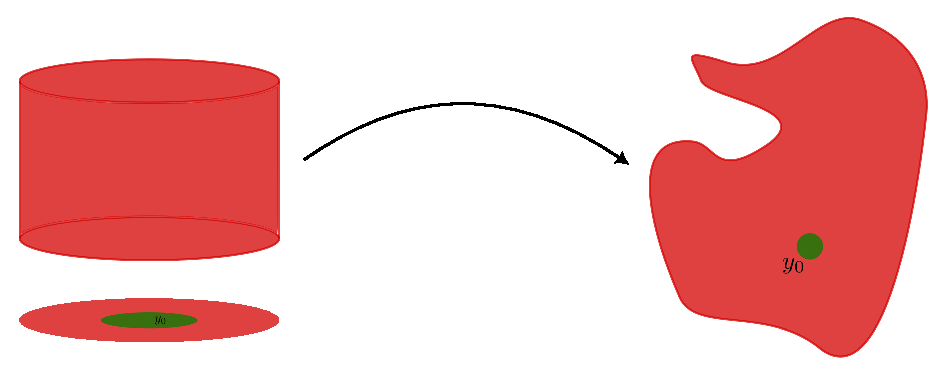
\includegraphics[scale=0.5]{Figures/equiv_homotopy.eps}
        \caption{La definici\'on de $g(x)$ que lleva a un cilindro a un disco
        perforado y rellena el hueco con $y_0$}.
        \label{fig_12}
    \end{figure}

    Suponga ahora que existe un extensi\'on $g:D^{n+1} \xrightarrow{} Y$ de $f$.
    Como  $S^n$ es subsespacio de  $D^{n+1}$, tenemos que $g \circ
    i=g|_{S^n}=f$. Sea $x_0 \in S^n$, y $k:x \xrightarrow{} f(x_0)$ una mapa
    constante. Defina $F:S^n \times I \xrightarrow{} Y$ dado por
    $F(x,t)=g((1-t)x+x_0t)$. Entonces $F$ es continua por composicion de mapas
    continuas, ademas $F(x,0)=g(x)=f(x)$, como $x \in S^n$, y
    $F(x,1)=g(x_0)=f(x_0)=k(x)$, como $x_0 \in S^n$. Por lo tanto, $F$ defina
    una homotopia entre  $f$ y  $k$.
\end{proof}

\begin{example}\label{}
    Considere $S^{n-1}$ y $D^n$ y considere la siguiente diagrama
    % https://q.uiver.app/?q=WzAsMyxbMCwwLCJTXntuLTF9Il0sWzMsMCwiU157bi0xfSJdLFswLDMsIkRebiJdLFswLDEsIjFfe1Nee24tMX19Il0sWzAsMiwiaSIsMl0sWzIsMSwiZyIsMix7InN0eWxlIjp7ImJvZHkiOnsibmFtZSI6ImRhc2hlZCJ9fX1dXQ==
    \[\begin{tikzcd}
        {S^{n-1}} &&& {S^{n-1}} \\
        \\
        \\
        {D^n}
        \arrow["{1_{S^{n-1}}}", from=1-1, to=1-4]
        \arrow["i"', from=1-1, to=4-1]
        \arrow["g"', dashed, from=4-1, to=1-4]
    \end{tikzcd}\]
    S\'i $g$ es una extensi\'on de $1_{S^{n-1}}$, entonces tenemos que  la
    diagrama es commutativa y que $g \circ i=1_{S^{n-1}}$; es decir que $g$ es
    una retracci\'on de  $S^{n-1}$, lo cual es imposible. As\'i que por la
    teorema anterior, $1_{S^{n-1}}$ no puede ser nulhomotopico.
\end{example}
